\documentclass[12pt, a4paper]{article} %mostra o tipo do documento
\setlength{\topmargin}{-.5in}
\setlength{\textheight}{9in}
\setlength{\textwidth}{6.3in}
\setlength{\oddsidemargin}{-.125in}
\setlength{\evensidemargin}{-.125in}
\usepackage[brazil]{babel} %permite escrever em português
\usepackage[utf8]{inputenc}
\usepackage[a4paper, textheight=260mm, textwidth=162mm]{geometry} %ajusta as margens
\usepackage[T1]{fontenc} %define a fonte das letras
\usepackage{color} %colore as letras
\usepackage{url} %inclui urls
\usepackage[pdfencoding=unicode]{hyperref} %transforma links em texto comum para clicar
\usepackage{amsmath, amssymb, amsthm, amsfonts} %permite fazer textos matemáticos
\usepackage{float} % permite mover tabelas e figuras para qualquer ponto da página
\usepackage{graphicx} %permite colocar imagens no documento

\title{Relatório EP3 - MAC0121}
\date{}
\author{João Gabriel Basi - $\text{N}^\circ$ USP: 9793801}
\begin{document}
\maketitle
\begin{enumerate}
\large
\item[1.]\textbf{O programa}
\normalsize\\[0.5cm]
O programa recebe um vetor desordenado de $n$ posições e o ordena usando 3-reversões. Quando é possível ordená-lo, o programa imprime uma sequencia de movimentos que fazem isso, quando não é possível, o programa imprime "Nao e possivel".\\[0.5cm]
\large
\item[2.]\textbf{As funções}
\normalsize\\[0.5cm]
O programa utiliza duas bibliotecas feitas por mim com algumas funções auxiliares:
\begin{itemize}
\item $mystack.h$: Define uma pilha e algumas funções sobre ela;
\item $myvector.h$: Tem funções que ajudam no manuseio de vetores e matrizes.
\end{itemize}
A função principal do programa é a $triSort$, que coordena como o vetor será ordenado. Para ordenar vetores com tamanhos ímpares ela utiliza as funções:
\begin{itemize}
\item $pMaior$: Recebe um vetor e seu tamanho e retorna a posição do maior elemento do vetor;
\item $triReversao$: Recebe um vetor, seu tamanho e uma posição e realiza uma 3-reversão na posição fornecida.
\end{itemize}
Já para vetores de tamanhos pares, ela utiliza as funções:
\begin{itemize}
\item $separa$: Recebe um vetor, seu tamanho e dois vetores com metade de seu tamanho e separa os elementos do vetor maior pela paridade de seus índices nos dois vetores menores;
\item $junta$: Faz o contrário da função $separa$, ou seja, volta os elementos dos vetores menores para o vetor maior intercalando-os;
\item $mergeSort$: Função de ordenação recursiva que recebe um vetor, o intervalo a ser ordenado, uma pilha e um coeficiente de paridade. Ordena o vetor normalmente utilizando um Merge Sort, calcula a posição relativa dos elementos movimentados no vetor original utilizando o coeficiente de paridade e as guarda na pilha.\\[2cm]
\end{itemize}
\large
\item[3.]\textbf{Métodos e otimizações}
\normalsize\\[0.5cm]
Para vetores com um número ímpar de posições, a cada passo eu identifico o maior número da parte desordenada do vetor utilizando a $pMaior$, se a paridade do índice dele for igual à paridade do índice da posição final, ele faz 3-reversões no elemento para frente até ele chegar na posição final, se for diferente, ele faz 3-reversões para trás até o número dar a volta no vetor e chegar na posição de destino e volta para arrumar os números que já tinham sido ordenados. Exemplo na imagem.
\small
\begin{center}
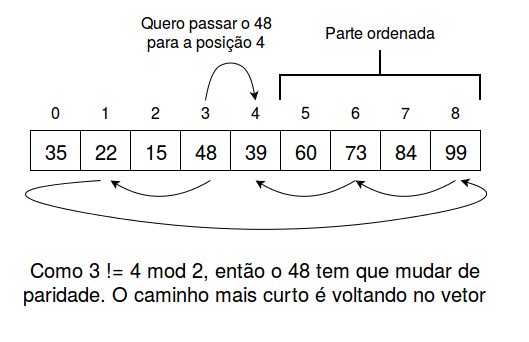
\includegraphics[scale=0.49]{vector13.png}\\
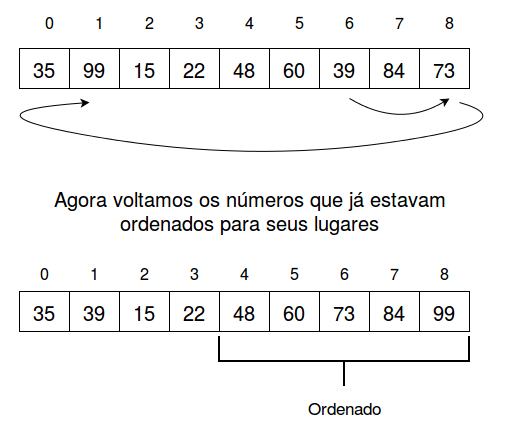
\includegraphics[scale=0.49]{vector23.png}\\
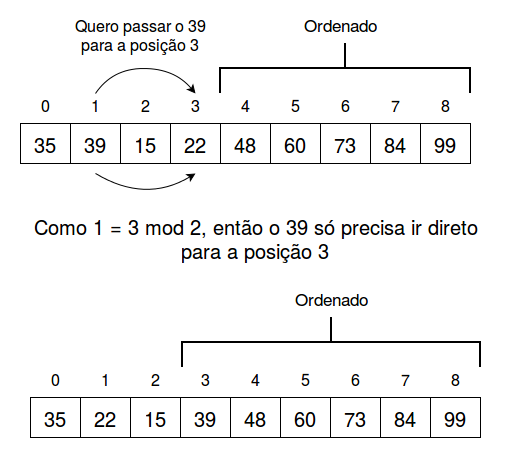
\includegraphics[scale=0.49]{vector32.png}\\
\end{center}
\normalsize
Como sempre é possível ordenar vetores ímpares, já que um número pode ir para qualquer posição do vetor, o programa imprime os movimentos feitos à medida que eles vão acontecendo.\\
Para vetores com um número par de posições, como não importa qual rotação sea feita, a paridade da posição de um elemento não muda, eu separei os números com índices pares e ímpares em dois vetores menores e os ordenei com um algoritmo de ordenação tradicional, já que nesses vetores uma 2-rotação é equivalente à uma 3-rotação no vetor original. Como é possível que o vetor seja impossível de ordenar, já que um número não pode ir para qualquer posição do vetor, eu guardo os movimentos feitos em uma pilha. Depois de ordenar-los eu junto eles de volta no vetor maior, se o vetor final estiver ordenado, o programa imprime os movimentos feitos, se não, ele imprime "Nao e possivel".\\[0.5cm]
\large
\item[5.]\textbf{Prós e contras}
\normalsize\\[0.5cm]
Prós:
\begin{itemize}
\item Ordena vetores pares em ordem O(nlogn) no pior caso;
\item 
\end{itemize}
Contras:
\begin{itemize}
\item Tem complexidade O(nlogn) para vetores pares ordenados também, por utilizar o merge sort;
\item O algoritmo de ordenação para ímpares é muito simples, por isso ele pode não achar os melhores movimentos que ordenam o vetor.
\end{itemize}
\end{enumerate}
\end{document}